% Created by tikzDevice version 0.10.1 on 2016-12-12 10:29:22
% !TEX encoding = UTF-8 Unicode
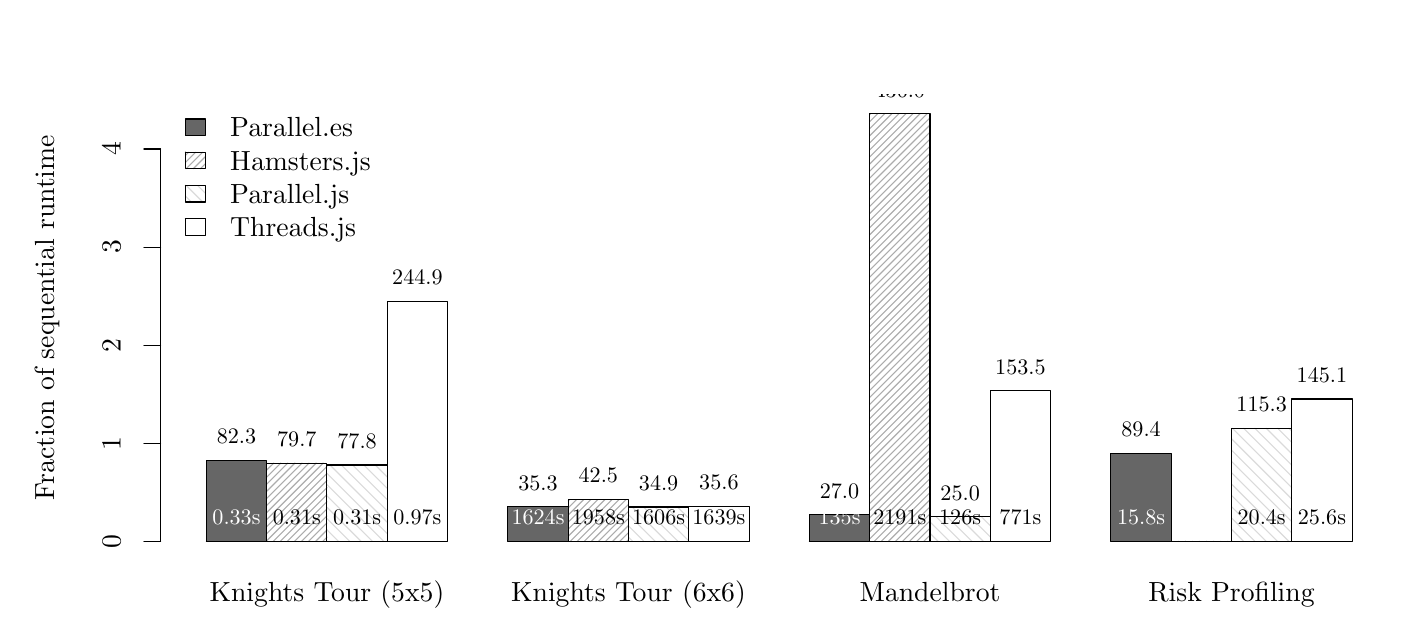
\begin{tikzpicture}[x=1pt,y=1pt]
\definecolor{fillColor}{RGB}{255,255,255}
\path[use as bounding box,fill=fillColor,fill opacity=0.00] (0,0) rectangle (495.15,209.58);
\begin{scope}
\path[clip] (  0.00,  0.00) rectangle (495.15,209.58);
\definecolor{fillColor}{gray}{0.40}

\path[fill=fillColor] ( 64.56, 24.00) --
	( 86.35, 24.00) --
	( 86.35, 53.16) --
	( 64.56, 53.16) --
	cycle;
\definecolor{drawColor}{RGB}{172,172,172}

\path[draw=drawColor,line width= 0.4pt,line join=round,line cap=round] ( 86.35, 49.70) -- ( 88.90, 52.24);

\path[draw=drawColor,line width= 0.4pt,line join=round,line cap=round] ( 86.35, 47.14) -- ( 91.45, 52.24);

\path[draw=drawColor,line width= 0.4pt,line join=round,line cap=round] ( 86.35, 44.59) -- ( 94.01, 52.24);

\path[draw=drawColor,line width= 0.4pt,line join=round,line cap=round] ( 86.35, 42.03) -- ( 96.56, 52.24);

\path[draw=drawColor,line width= 0.4pt,line join=round,line cap=round] ( 86.35, 39.48) -- ( 99.12, 52.24);

\path[draw=drawColor,line width= 0.4pt,line join=round,line cap=round] ( 86.35, 36.92) -- (101.67, 52.24);

\path[draw=drawColor,line width= 0.4pt,line join=round,line cap=round] ( 86.35, 34.36) -- (104.23, 52.24);

\path[draw=drawColor,line width= 0.4pt,line join=round,line cap=round] ( 86.35, 31.81) -- (106.78, 52.24);

\path[draw=drawColor,line width= 0.4pt,line join=round,line cap=round] ( 86.35, 29.25) -- (108.14, 51.05);

\path[draw=drawColor,line width= 0.4pt,line join=round,line cap=round] ( 86.35, 26.70) -- (108.14, 48.49);

\path[draw=drawColor,line width= 0.4pt,line join=round,line cap=round] ( 86.35, 24.14) -- (108.14, 45.94);

\path[draw=drawColor,line width= 0.4pt,line join=round,line cap=round] ( 88.76, 24.00) -- (108.14, 43.38);

\path[draw=drawColor,line width= 0.4pt,line join=round,line cap=round] ( 91.32, 24.00) -- (108.14, 40.82);

\path[draw=drawColor,line width= 0.4pt,line join=round,line cap=round] ( 93.87, 24.00) -- (108.14, 38.27);

\path[draw=drawColor,line width= 0.4pt,line join=round,line cap=round] ( 96.43, 24.00) -- (108.14, 35.71);

\path[draw=drawColor,line width= 0.4pt,line join=round,line cap=round] ( 98.98, 24.00) -- (108.14, 33.16);

\path[draw=drawColor,line width= 0.4pt,line join=round,line cap=round] (101.54, 24.00) -- (108.14, 30.60);

\path[draw=drawColor,line width= 0.4pt,line join=round,line cap=round] (104.09, 24.00) -- (108.14, 28.05);

\path[draw=drawColor,line width= 0.4pt,line join=round,line cap=round] (106.65, 24.00) -- (108.14, 25.49);
\definecolor{drawColor}{RGB}{218,218,218}

\path[draw=drawColor,line width= 0.4pt,line join=round,line cap=round] (108.18, 24.00) -- (108.14, 24.04);

\path[draw=drawColor,line width= 0.4pt,line join=round,line cap=round] (112.27, 24.00) -- (108.14, 28.13);

\path[draw=drawColor,line width= 0.4pt,line join=round,line cap=round] (116.36, 24.00) -- (108.14, 32.22);

\path[draw=drawColor,line width= 0.4pt,line join=round,line cap=round] (120.45, 24.00) -- (108.14, 36.30);

\path[draw=drawColor,line width= 0.4pt,line join=round,line cap=round] (124.53, 24.00) -- (108.14, 40.39);

\path[draw=drawColor,line width= 0.4pt,line join=round,line cap=round] (128.62, 24.00) -- (108.14, 44.48);

\path[draw=drawColor,line width= 0.4pt,line join=round,line cap=round] (129.93, 26.78) -- (108.14, 48.57);

\path[draw=drawColor,line width= 0.4pt,line join=round,line cap=round] (129.93, 30.87) -- (109.24, 51.56);

\path[draw=drawColor,line width= 0.4pt,line join=round,line cap=round] (129.93, 34.95) -- (113.33, 51.56);

\path[draw=drawColor,line width= 0.4pt,line join=round,line cap=round] (129.93, 39.04) -- (117.41, 51.56);

\path[draw=drawColor,line width= 0.4pt,line join=round,line cap=round] (129.93, 43.13) -- (121.50, 51.56);

\path[draw=drawColor,line width= 0.4pt,line join=round,line cap=round] (129.93, 47.22) -- (125.59, 51.56);

\path[draw=drawColor,line width= 0.4pt,line join=round,line cap=round] (129.93, 51.31) -- (129.68, 51.56);

\path[fill=fillColor] (173.51, 24.00) --
	(195.31, 24.00) --
	(195.31, 36.50) --
	(173.51, 36.50) --
	cycle;
\definecolor{drawColor}{RGB}{172,172,172}

\path[draw=drawColor,line width= 0.4pt,line join=round,line cap=round] (195.31, 38.56) -- (195.82, 39.08);

\path[draw=drawColor,line width= 0.4pt,line join=round,line cap=round] (195.31, 36.00) -- (198.38, 39.08);

\path[draw=drawColor,line width= 0.4pt,line join=round,line cap=round] (195.31, 33.45) -- (200.93, 39.08);

\path[draw=drawColor,line width= 0.4pt,line join=round,line cap=round] (195.31, 30.89) -- (203.49, 39.08);

\path[draw=drawColor,line width= 0.4pt,line join=round,line cap=round] (195.31, 28.34) -- (206.04, 39.08);

\path[draw=drawColor,line width= 0.4pt,line join=round,line cap=round] (195.31, 25.78) -- (208.60, 39.08);

\path[draw=drawColor,line width= 0.4pt,line join=round,line cap=round] (196.08, 24.00) -- (211.15, 39.08);

\path[draw=drawColor,line width= 0.4pt,line join=round,line cap=round] (198.63, 24.00) -- (213.71, 39.08);

\path[draw=drawColor,line width= 0.4pt,line join=round,line cap=round] (201.19, 24.00) -- (216.26, 39.08);

\path[draw=drawColor,line width= 0.4pt,line join=round,line cap=round] (203.74, 24.00) -- (217.10, 37.35);

\path[draw=drawColor,line width= 0.4pt,line join=round,line cap=round] (206.30, 24.00) -- (217.10, 34.80);

\path[draw=drawColor,line width= 0.4pt,line join=round,line cap=round] (208.85, 24.00) -- (217.10, 32.24);

\path[draw=drawColor,line width= 0.4pt,line join=round,line cap=round] (211.41, 24.00) -- (217.10, 29.69);

\path[draw=drawColor,line width= 0.4pt,line join=round,line cap=round] (213.96, 24.00) -- (217.10, 27.13);

\path[draw=drawColor,line width= 0.4pt,line join=round,line cap=round] (216.52, 24.00) -- (217.10, 24.58);
\definecolor{drawColor}{RGB}{218,218,218}

\path[draw=drawColor,line width= 0.4pt,line join=round,line cap=round] (218.56, 24.00) -- (217.10, 25.47);

\path[draw=drawColor,line width= 0.4pt,line join=round,line cap=round] (222.65, 24.00) -- (217.10, 29.55);

\path[draw=drawColor,line width= 0.4pt,line join=round,line cap=round] (226.74, 24.00) -- (217.10, 33.64);

\path[draw=drawColor,line width= 0.4pt,line join=round,line cap=round] (230.83, 24.00) -- (218.46, 36.36);

\path[draw=drawColor,line width= 0.4pt,line join=round,line cap=round] (234.92, 24.00) -- (222.55, 36.36);

\path[draw=drawColor,line width= 0.4pt,line join=round,line cap=round] (238.89, 24.12) -- (226.64, 36.36);

\path[draw=drawColor,line width= 0.4pt,line join=round,line cap=round] (238.89, 28.21) -- (230.73, 36.36);

\path[draw=drawColor,line width= 0.4pt,line join=round,line cap=round] (238.89, 32.29) -- (234.82, 36.36);

\path[fill=fillColor] (282.47, 24.00) --
	(304.26, 24.00) --
	(304.26, 33.56) --
	(282.47, 33.56) --
	cycle;
\definecolor{drawColor}{RGB}{172,172,172}

\path[draw=drawColor,line width= 0.4pt,line join=round,line cap=round] (304.26,178.17) -- (304.58,178.50);

\path[draw=drawColor,line width= 0.4pt,line join=round,line cap=round] (304.26,175.62) -- (307.14,178.50);

\path[draw=drawColor,line width= 0.4pt,line join=round,line cap=round] (304.26,173.06) -- (309.69,178.50);

\path[draw=drawColor,line width= 0.4pt,line join=round,line cap=round] (304.26,170.51) -- (312.25,178.50);

\path[draw=drawColor,line width= 0.4pt,line join=round,line cap=round] (304.26,167.95) -- (314.80,178.50);

\path[draw=drawColor,line width= 0.4pt,line join=round,line cap=round] (304.26,165.40) -- (317.36,178.50);

\path[draw=drawColor,line width= 0.4pt,line join=round,line cap=round] (304.26,162.84) -- (319.91,178.50);

\path[draw=drawColor,line width= 0.4pt,line join=round,line cap=round] (304.26,160.29) -- (322.47,178.50);

\path[draw=drawColor,line width= 0.4pt,line join=round,line cap=round] (304.26,157.73) -- (325.02,178.50);

\path[draw=drawColor,line width= 0.4pt,line join=round,line cap=round] (304.26,155.18) -- (326.05,176.97);

\path[draw=drawColor,line width= 0.4pt,line join=round,line cap=round] (304.26,152.62) -- (326.05,174.41);

\path[draw=drawColor,line width= 0.4pt,line join=round,line cap=round] (304.26,150.07) -- (326.05,171.86);

\path[draw=drawColor,line width= 0.4pt,line join=round,line cap=round] (304.26,147.51) -- (326.05,169.30);

\path[draw=drawColor,line width= 0.4pt,line join=round,line cap=round] (304.26,144.96) -- (326.05,166.75);

\path[draw=drawColor,line width= 0.4pt,line join=round,line cap=round] (304.26,142.40) -- (326.05,164.19);

\path[draw=drawColor,line width= 0.4pt,line join=round,line cap=round] (304.26,139.85) -- (326.05,161.64);

\path[draw=drawColor,line width= 0.4pt,line join=round,line cap=round] (304.26,137.29) -- (326.05,159.08);

\path[draw=drawColor,line width= 0.4pt,line join=round,line cap=round] (304.26,134.74) -- (326.05,156.53);

\path[draw=drawColor,line width= 0.4pt,line join=round,line cap=round] (304.26,132.18) -- (326.05,153.97);

\path[draw=drawColor,line width= 0.4pt,line join=round,line cap=round] (304.26,129.63) -- (326.05,151.42);

\path[draw=drawColor,line width= 0.4pt,line join=round,line cap=round] (304.26,127.07) -- (326.05,148.86);

\path[draw=drawColor,line width= 0.4pt,line join=round,line cap=round] (304.26,124.52) -- (326.05,146.31);

\path[draw=drawColor,line width= 0.4pt,line join=round,line cap=round] (304.26,121.96) -- (326.05,143.75);

\path[draw=drawColor,line width= 0.4pt,line join=round,line cap=round] (304.26,119.41) -- (326.05,141.20);

\path[draw=drawColor,line width= 0.4pt,line join=round,line cap=round] (304.26,116.85) -- (326.05,138.64);

\path[draw=drawColor,line width= 0.4pt,line join=round,line cap=round] (304.26,114.30) -- (326.05,136.09);

\path[draw=drawColor,line width= 0.4pt,line join=round,line cap=round] (304.26,111.74) -- (326.05,133.53);

\path[draw=drawColor,line width= 0.4pt,line join=round,line cap=round] (304.26,109.19) -- (326.05,130.98);

\path[draw=drawColor,line width= 0.4pt,line join=round,line cap=round] (304.26,106.63) -- (326.05,128.42);

\path[draw=drawColor,line width= 0.4pt,line join=round,line cap=round] (304.26,104.08) -- (326.05,125.87);

\path[draw=drawColor,line width= 0.4pt,line join=round,line cap=round] (304.26,101.52) -- (326.05,123.31);

\path[draw=drawColor,line width= 0.4pt,line join=round,line cap=round] (304.26, 98.96) -- (326.05,120.76);

\path[draw=drawColor,line width= 0.4pt,line join=round,line cap=round] (304.26, 96.41) -- (326.05,118.20);

\path[draw=drawColor,line width= 0.4pt,line join=round,line cap=round] (304.26, 93.85) -- (326.05,115.65);

\path[draw=drawColor,line width= 0.4pt,line join=round,line cap=round] (304.26, 91.30) -- (326.05,113.09);

\path[draw=drawColor,line width= 0.4pt,line join=round,line cap=round] (304.26, 88.74) -- (326.05,110.54);

\path[draw=drawColor,line width= 0.4pt,line join=round,line cap=round] (304.26, 86.19) -- (326.05,107.98);

\path[draw=drawColor,line width= 0.4pt,line join=round,line cap=round] (304.26, 83.63) -- (326.05,105.43);

\path[draw=drawColor,line width= 0.4pt,line join=round,line cap=round] (304.26, 81.08) -- (326.05,102.87);

\path[draw=drawColor,line width= 0.4pt,line join=round,line cap=round] (304.26, 78.52) -- (326.05,100.31);

\path[draw=drawColor,line width= 0.4pt,line join=round,line cap=round] (304.26, 75.97) -- (326.05, 97.76);

\path[draw=drawColor,line width= 0.4pt,line join=round,line cap=round] (304.26, 73.41) -- (326.05, 95.20);

\path[draw=drawColor,line width= 0.4pt,line join=round,line cap=round] (304.26, 70.86) -- (326.05, 92.65);

\path[draw=drawColor,line width= 0.4pt,line join=round,line cap=round] (304.26, 68.30) -- (326.05, 90.09);

\path[draw=drawColor,line width= 0.4pt,line join=round,line cap=round] (304.26, 65.75) -- (326.05, 87.54);

\path[draw=drawColor,line width= 0.4pt,line join=round,line cap=round] (304.26, 63.19) -- (326.05, 84.98);

\path[draw=drawColor,line width= 0.4pt,line join=round,line cap=round] (304.26, 60.64) -- (326.05, 82.43);

\path[draw=drawColor,line width= 0.4pt,line join=round,line cap=round] (304.26, 58.08) -- (326.05, 79.87);

\path[draw=drawColor,line width= 0.4pt,line join=round,line cap=round] (304.26, 55.53) -- (326.05, 77.32);

\path[draw=drawColor,line width= 0.4pt,line join=round,line cap=round] (304.26, 52.97) -- (326.05, 74.76);

\path[draw=drawColor,line width= 0.4pt,line join=round,line cap=round] (304.26, 50.42) -- (326.05, 72.21);

\path[draw=drawColor,line width= 0.4pt,line join=round,line cap=round] (304.26, 47.86) -- (326.05, 69.65);

\path[draw=drawColor,line width= 0.4pt,line join=round,line cap=round] (304.26, 45.31) -- (326.05, 67.10);

\path[draw=drawColor,line width= 0.4pt,line join=round,line cap=round] (304.26, 42.75) -- (326.05, 64.54);

\path[draw=drawColor,line width= 0.4pt,line join=round,line cap=round] (304.26, 40.20) -- (326.05, 61.99);

\path[draw=drawColor,line width= 0.4pt,line join=round,line cap=round] (304.26, 37.64) -- (326.05, 59.43);

\path[draw=drawColor,line width= 0.4pt,line join=round,line cap=round] (304.26, 35.09) -- (326.05, 56.88);

\path[draw=drawColor,line width= 0.4pt,line join=round,line cap=round] (304.26, 32.53) -- (326.05, 54.32);

\path[draw=drawColor,line width= 0.4pt,line join=round,line cap=round] (304.26, 29.98) -- (326.05, 51.77);

\path[draw=drawColor,line width= 0.4pt,line join=round,line cap=round] (304.26, 27.42) -- (326.05, 49.21);

\path[draw=drawColor,line width= 0.4pt,line join=round,line cap=round] (304.26, 24.87) -- (326.05, 46.66);

\path[draw=drawColor,line width= 0.4pt,line join=round,line cap=round] (305.95, 24.00) -- (326.05, 44.10);

\path[draw=drawColor,line width= 0.4pt,line join=round,line cap=round] (308.50, 24.00) -- (326.05, 41.55);

\path[draw=drawColor,line width= 0.4pt,line join=round,line cap=round] (311.06, 24.00) -- (326.05, 38.99);

\path[draw=drawColor,line width= 0.4pt,line join=round,line cap=round] (313.61, 24.00) -- (326.05, 36.44);

\path[draw=drawColor,line width= 0.4pt,line join=round,line cap=round] (316.17, 24.00) -- (326.05, 33.88);

\path[draw=drawColor,line width= 0.4pt,line join=round,line cap=round] (318.72, 24.00) -- (326.05, 31.33);

\path[draw=drawColor,line width= 0.4pt,line join=round,line cap=round] (321.28, 24.00) -- (326.05, 28.77);

\path[draw=drawColor,line width= 0.4pt,line join=round,line cap=round] (323.83, 24.00) -- (326.05, 26.22);
\definecolor{drawColor}{RGB}{218,218,218}

\path[draw=drawColor,line width= 0.4pt,line join=round,line cap=round] (328.94, 24.00) -- (326.05, 26.89);

\path[draw=drawColor,line width= 0.4pt,line join=round,line cap=round] (333.03, 24.00) -- (326.05, 30.98);

\path[draw=drawColor,line width= 0.4pt,line join=round,line cap=round] (337.12, 24.00) -- (328.25, 32.87);

\path[draw=drawColor,line width= 0.4pt,line join=round,line cap=round] (341.21, 24.00) -- (332.34, 32.87);

\path[draw=drawColor,line width= 0.4pt,line join=round,line cap=round] (345.30, 24.00) -- (336.43, 32.87);

\path[draw=drawColor,line width= 0.4pt,line join=round,line cap=round] (347.84, 25.54) -- (340.52, 32.87);

\path[draw=drawColor,line width= 0.4pt,line join=round,line cap=round] (347.84, 29.63) -- (344.61, 32.87);

\path[fill=fillColor] (391.42, 24.00) --
	(413.21, 24.00) --
	(413.21, 55.69) --
	(391.42, 55.69) --
	cycle;
\definecolor{drawColor}{RGB}{172,172,172}

\path[draw=drawColor,line width= 0.4pt,line join=round,line cap=round] (413.26, 24.00) -- (413.26, 24.00);

\path[draw=drawColor,line width= 0.4pt,line join=round,line cap=round] (415.82, 24.00) -- (415.82, 24.00);

\path[draw=drawColor,line width= 0.4pt,line join=round,line cap=round] (418.37, 24.00) -- (418.37, 24.00);

\path[draw=drawColor,line width= 0.4pt,line join=round,line cap=round] (420.93, 24.00) -- (420.93, 24.00);

\path[draw=drawColor,line width= 0.4pt,line join=round,line cap=round] (423.48, 24.00) -- (423.48, 24.00);

\path[draw=drawColor,line width= 0.4pt,line join=round,line cap=round] (426.04, 24.00) -- (426.04, 24.00);

\path[draw=drawColor,line width= 0.4pt,line join=round,line cap=round] (428.59, 24.00) -- (428.59, 24.00);

\path[draw=drawColor,line width= 0.4pt,line join=round,line cap=round] (431.15, 24.00) -- (431.15, 24.00);

\path[draw=drawColor,line width= 0.4pt,line join=round,line cap=round] (433.71, 24.00) -- (433.71, 24.00);
\definecolor{drawColor}{RGB}{218,218,218}

\path[draw=drawColor,line width= 0.4pt,line join=round,line cap=round] (435.24, 24.00) -- (435.00, 24.23);

\path[draw=drawColor,line width= 0.4pt,line join=round,line cap=round] (439.33, 24.00) -- (435.00, 28.32);

\path[draw=drawColor,line width= 0.4pt,line join=round,line cap=round] (443.41, 24.00) -- (435.00, 32.41);

\path[draw=drawColor,line width= 0.4pt,line join=round,line cap=round] (447.50, 24.00) -- (435.00, 36.50);

\path[draw=drawColor,line width= 0.4pt,line join=round,line cap=round] (451.59, 24.00) -- (435.00, 40.59);

\path[draw=drawColor,line width= 0.4pt,line join=round,line cap=round] (455.68, 24.00) -- (435.00, 44.67);

\path[draw=drawColor,line width= 0.4pt,line join=round,line cap=round] (456.80, 26.97) -- (435.00, 48.76);

\path[draw=drawColor,line width= 0.4pt,line join=round,line cap=round] (456.80, 31.06) -- (435.00, 52.85);

\path[draw=drawColor,line width= 0.4pt,line join=round,line cap=round] (456.80, 35.15) -- (435.00, 56.94);

\path[draw=drawColor,line width= 0.4pt,line join=round,line cap=round] (456.80, 39.24) -- (435.00, 61.03);

\path[draw=drawColor,line width= 0.4pt,line join=round,line cap=round] (456.80, 43.33) -- (435.26, 64.86);

\path[draw=drawColor,line width= 0.4pt,line join=round,line cap=round] (456.80, 47.41) -- (439.35, 64.86);

\path[draw=drawColor,line width= 0.4pt,line join=round,line cap=round] (456.80, 51.50) -- (443.43, 64.86);

\path[draw=drawColor,line width= 0.4pt,line join=round,line cap=round] (456.80, 55.59) -- (447.52, 64.86);

\path[draw=drawColor,line width= 0.4pt,line join=round,line cap=round] (456.80, 59.68) -- (451.61, 64.86);

\path[draw=drawColor,line width= 0.4pt,line join=round,line cap=round] (456.80, 63.77) -- (455.70, 64.86);
\definecolor{drawColor}{RGB}{0,0,0}

\path[draw=drawColor,line width= 0.4pt,line join=round,line cap=round] ( 64.56, 24.00) --
	( 86.35, 24.00) --
	( 86.35, 53.16) --
	( 64.56, 53.16) --
	( 64.56, 24.00);

\path[draw=drawColor,line width= 0.4pt,line join=round,line cap=round] ( 86.35, 24.00) --
	(108.14, 24.00) --
	(108.14, 52.24) --
	( 86.35, 52.24) --
	( 86.35, 24.00);

\path[draw=drawColor,line width= 0.4pt,line join=round,line cap=round] (108.14, 24.00) --
	(129.93, 24.00) --
	(129.93, 51.56) --
	(108.14, 51.56) --
	(108.14, 24.00);

\path[draw=drawColor,line width= 0.4pt,line join=round,line cap=round] (129.93, 24.00) --
	(151.72, 24.00) --
	(151.72,110.77) --
	(129.93,110.77) --
	(129.93, 24.00);

\path[draw=drawColor,line width= 0.4pt,line join=round,line cap=round] (173.51, 24.00) --
	(195.31, 24.00) --
	(195.31, 36.50) --
	(173.51, 36.50) --
	(173.51, 24.00);

\path[draw=drawColor,line width= 0.4pt,line join=round,line cap=round] (195.31, 24.00) --
	(217.10, 24.00) --
	(217.10, 39.08) --
	(195.31, 39.08) --
	(195.31, 24.00);

\path[draw=drawColor,line width= 0.4pt,line join=round,line cap=round] (217.10, 24.00) --
	(238.89, 24.00) --
	(238.89, 36.36) --
	(217.10, 36.36) --
	(217.10, 24.00);

\path[draw=drawColor,line width= 0.4pt,line join=round,line cap=round] (238.89, 24.00) --
	(260.68, 24.00) --
	(260.68, 36.62) --
	(238.89, 36.62) --
	(238.89, 24.00);

\path[draw=drawColor,line width= 0.4pt,line join=round,line cap=round] (282.47, 24.00) --
	(304.26, 24.00) --
	(304.26, 33.56) --
	(282.47, 33.56) --
	(282.47, 24.00);

\path[draw=drawColor,line width= 0.4pt,line join=round,line cap=round] (304.26, 24.00) --
	(326.05, 24.00) --
	(326.05,178.50) --
	(304.26,178.50) --
	(304.26, 24.00);

\path[draw=drawColor,line width= 0.4pt,line join=round,line cap=round] (326.05, 24.00) --
	(347.84, 24.00) --
	(347.84, 32.87) --
	(326.05, 32.87) --
	(326.05, 24.00);

\path[draw=drawColor,line width= 0.4pt,line join=round,line cap=round] (347.84, 24.00) --
	(369.63, 24.00) --
	(369.63, 78.37) --
	(347.84, 78.37) --
	(347.84, 24.00);

\path[draw=drawColor,line width= 0.4pt,line join=round,line cap=round] (391.42, 24.00) --
	(413.21, 24.00) --
	(413.21, 55.69) --
	(391.42, 55.69) --
	(391.42, 24.00);

\path[draw=drawColor,line width= 0.4pt,line join=round,line cap=round] (413.21, 24.00) --
	(435.00, 24.00) --
	(413.21, 24.00);

\path[draw=drawColor,line width= 0.4pt,line join=round,line cap=round] (435.00, 24.00) --
	(456.80, 24.00) --
	(456.80, 64.86) --
	(435.00, 64.86) --
	(435.00, 24.00);

\path[draw=drawColor,line width= 0.4pt,line join=round,line cap=round] (456.80, 24.00) --
	(478.59, 24.00) --
	(478.59, 75.40) --
	(456.80, 75.40) --
	(456.80, 24.00);
\end{scope}
\begin{scope}
\path[clip] (  0.00,  0.00) rectangle (495.15,209.58);
\definecolor{drawColor}{RGB}{0,0,0}

\node[text=drawColor,anchor=base,inner sep=0pt, outer sep=0pt, scale=  1.00] at (108.14,  2.40) {Knights Tour (5x5)};

\node[text=drawColor,anchor=base,inner sep=0pt, outer sep=0pt, scale=  1.00] at (217.10,  2.40) {Knights Tour (6x6)};

\node[text=drawColor,anchor=base,inner sep=0pt, outer sep=0pt, scale=  1.00] at (326.05,  2.40) {Mandelbrot};

\node[text=drawColor,anchor=base,inner sep=0pt, outer sep=0pt, scale=  1.00] at (435.00,  2.40) {Risk Profiling};
\end{scope}
\begin{scope}
\path[clip] (  0.00,  0.00) rectangle (495.15,209.58);
\definecolor{drawColor}{RGB}{0,0,0}

\node[text=drawColor,rotate= 90.00,anchor=base,inner sep=0pt, outer sep=0pt, scale=  1.00] at (  9.60,104.79) {Fraction of sequential runtime};
\end{scope}
\begin{scope}
\path[clip] (  0.00,  0.00) rectangle (495.15,209.58);
\definecolor{drawColor}{RGB}{0,0,0}

\path[draw=drawColor,line width= 0.4pt,line join=round,line cap=round] ( 48.00, 24.00) -- ( 48.00,165.73);

\path[draw=drawColor,line width= 0.4pt,line join=round,line cap=round] ( 48.00, 24.00) -- ( 42.00, 24.00);

\path[draw=drawColor,line width= 0.4pt,line join=round,line cap=round] ( 48.00, 59.43) -- ( 42.00, 59.43);

\path[draw=drawColor,line width= 0.4pt,line join=round,line cap=round] ( 48.00, 94.86) -- ( 42.00, 94.86);

\path[draw=drawColor,line width= 0.4pt,line join=round,line cap=round] ( 48.00,130.30) -- ( 42.00,130.30);

\path[draw=drawColor,line width= 0.4pt,line join=round,line cap=round] ( 48.00,165.73) -- ( 42.00,165.73);

\node[text=drawColor,rotate= 90.00,anchor=base,inner sep=0pt, outer sep=0pt, scale=  1.00] at ( 33.60, 24.00) {0};

\node[text=drawColor,rotate= 90.00,anchor=base,inner sep=0pt, outer sep=0pt, scale=  1.00] at ( 33.60, 59.43) {1};

\node[text=drawColor,rotate= 90.00,anchor=base,inner sep=0pt, outer sep=0pt, scale=  1.00] at ( 33.60, 94.86) {2};

\node[text=drawColor,rotate= 90.00,anchor=base,inner sep=0pt, outer sep=0pt, scale=  1.00] at ( 33.60,130.30) {3};

\node[text=drawColor,rotate= 90.00,anchor=base,inner sep=0pt, outer sep=0pt, scale=  1.00] at ( 33.60,165.73) {4};
\end{scope}
\begin{scope}
\path[clip] ( 48.00, 24.00) rectangle (495.15,185.58);
\definecolor{fillColor}{gray}{0.40}

\path[fill=fillColor] ( 57.00,176.58) --
	( 64.20,176.58) --
	( 64.20,170.58) --
	( 57.00,170.58) --
	cycle;
\definecolor{drawColor}{RGB}{172,172,172}

\path[draw=drawColor,line width= 0.4pt,line join=round,line cap=round] ( 57.00,163.43) -- ( 58.15,164.58);

\path[draw=drawColor,line width= 0.4pt,line join=round,line cap=round] ( 57.00,160.88) -- ( 60.71,164.58);

\path[draw=drawColor,line width= 0.4pt,line join=round,line cap=round] ( 57.26,158.58) -- ( 63.26,164.58);

\path[draw=drawColor,line width= 0.4pt,line join=round,line cap=round] ( 59.82,158.58) -- ( 64.20,162.97);

\path[draw=drawColor,line width= 0.4pt,line join=round,line cap=round] ( 62.37,158.58) -- ( 64.20,160.41);
\definecolor{drawColor}{RGB}{218,218,218}

\path[draw=drawColor,line width= 0.4pt,line join=round,line cap=round] ( 59.19,146.58) -- ( 57.00,148.77);

\path[draw=drawColor,line width= 0.4pt,line join=round,line cap=round] ( 63.27,146.58) -- ( 57.27,152.58);

\path[draw=drawColor,line width= 0.4pt,line join=round,line cap=round] ( 64.20,149.75) -- ( 61.36,152.58);
\definecolor{drawColor}{RGB}{0,0,0}

\path[draw=drawColor,line width= 0.4pt,line join=round,line cap=round] ( 57.00,176.58) --
	( 64.20,176.58) --
	( 64.20,170.58) --
	( 57.00,170.58) --
	( 57.00,176.58);

\path[draw=drawColor,line width= 0.4pt,line join=round,line cap=round] ( 57.00,164.58) --
	( 64.20,164.58) --
	( 64.20,158.58) --
	( 57.00,158.58) --
	( 57.00,164.58);

\path[draw=drawColor,line width= 0.4pt,line join=round,line cap=round] ( 57.00,152.58) --
	( 64.20,152.58) --
	( 64.20,146.58) --
	( 57.00,146.58) --
	( 57.00,152.58);

\path[draw=drawColor,line width= 0.4pt,line join=round,line cap=round] ( 57.00,140.58) --
	( 64.20,140.58) --
	( 64.20,134.58) --
	( 57.00,134.58) --
	( 57.00,140.58);

\node[text=drawColor,anchor=base west,inner sep=0pt, outer sep=0pt, scale=  1.00] at ( 73.20,170.14) {Parallel.es};

\node[text=drawColor,anchor=base west,inner sep=0pt, outer sep=0pt, scale=  1.00] at ( 73.20,158.14) {Hamsters.js};

\node[text=drawColor,anchor=base west,inner sep=0pt, outer sep=0pt, scale=  1.00] at ( 73.20,146.14) {Parallel.js};

\node[text=drawColor,anchor=base west,inner sep=0pt, outer sep=0pt, scale=  1.00] at ( 73.20,134.14) {Threads.js};

\node[text=drawColor,anchor=base,inner sep=0pt, outer sep=0pt, scale=  0.80] at ( 75.46, 59.16) {82.3};

\node[text=drawColor,anchor=base,inner sep=0pt, outer sep=0pt, scale=  0.80] at ( 97.25, 58.24) {79.7};

\node[text=drawColor,anchor=base,inner sep=0pt, outer sep=0pt, scale=  0.80] at (119.04, 57.56) {77.8};

\node[text=drawColor,anchor=base,inner sep=0pt, outer sep=0pt, scale=  0.80] at (140.83,116.77) {244.9};

\node[text=drawColor,anchor=base,inner sep=0pt, outer sep=0pt, scale=  0.80] at (184.41, 42.50) {35.3};

\node[text=drawColor,anchor=base,inner sep=0pt, outer sep=0pt, scale=  0.80] at (206.20, 45.08) {42.5};

\node[text=drawColor,anchor=base,inner sep=0pt, outer sep=0pt, scale=  0.80] at (227.99, 42.36) {34.9};

\node[text=drawColor,anchor=base,inner sep=0pt, outer sep=0pt, scale=  0.80] at (249.78, 42.62) {35.6};

\node[text=drawColor,anchor=base,inner sep=0pt, outer sep=0pt, scale=  0.80] at (293.36, 39.56) {27.0};

\node[text=drawColor,anchor=base,inner sep=0pt, outer sep=0pt, scale=  0.80] at (315.16,184.50) {436.0};

\node[text=drawColor,anchor=base,inner sep=0pt, outer sep=0pt, scale=  0.80] at (336.95, 38.87) {25.0};

\node[text=drawColor,anchor=base,inner sep=0pt, outer sep=0pt, scale=  0.80] at (358.74, 84.37) {153.5};

\node[text=drawColor,anchor=base,inner sep=0pt, outer sep=0pt, scale=  0.80] at (402.32, 61.69) {89.4};

\node[text=drawColor,anchor=base,inner sep=0pt, outer sep=0pt, scale=  0.80] at (445.90, 70.86) {115.3};

\node[text=drawColor,anchor=base,inner sep=0pt, outer sep=0pt, scale=  0.80] at (467.69, 81.40) {145.1};
\definecolor{drawColor}{RGB}{255,255,255}

\node[text=drawColor,anchor=base,inner sep=0pt, outer sep=0pt, scale=  0.80] at ( 75.46, 30.00) {0.33s};
\definecolor{drawColor}{RGB}{0,0,0}

\node[text=drawColor,anchor=base,inner sep=0pt, outer sep=0pt, scale=  0.80] at ( 97.25, 30.00) {0.31s};

\node[text=drawColor,anchor=base,inner sep=0pt, outer sep=0pt, scale=  0.80] at (119.04, 30.00) {0.31s};

\node[text=drawColor,anchor=base,inner sep=0pt, outer sep=0pt, scale=  0.80] at (140.83, 30.00) {0.97s};
\definecolor{drawColor}{RGB}{255,255,255}

\node[text=drawColor,anchor=base,inner sep=0pt, outer sep=0pt, scale=  0.80] at (184.41, 30.00) {1624s};
\definecolor{drawColor}{RGB}{0,0,0}

\node[text=drawColor,anchor=base,inner sep=0pt, outer sep=0pt, scale=  0.80] at (206.20, 30.00) {1958s};

\node[text=drawColor,anchor=base,inner sep=0pt, outer sep=0pt, scale=  0.80] at (227.99, 30.00) {1606s};

\node[text=drawColor,anchor=base,inner sep=0pt, outer sep=0pt, scale=  0.80] at (249.78, 30.00) {1639s};
\definecolor{drawColor}{RGB}{255,255,255}

\node[text=drawColor,anchor=base,inner sep=0pt, outer sep=0pt, scale=  0.80] at (293.36, 30.00) {135s};
\definecolor{drawColor}{RGB}{0,0,0}

\node[text=drawColor,anchor=base,inner sep=0pt, outer sep=0pt, scale=  0.80] at (315.16, 30.00) {2191s};

\node[text=drawColor,anchor=base,inner sep=0pt, outer sep=0pt, scale=  0.80] at (336.95, 30.00) {126s};

\node[text=drawColor,anchor=base,inner sep=0pt, outer sep=0pt, scale=  0.80] at (358.74, 30.00) {771s};
\definecolor{drawColor}{RGB}{255,255,255}

\node[text=drawColor,anchor=base,inner sep=0pt, outer sep=0pt, scale=  0.80] at (402.32, 30.00) {15.8s};
\definecolor{drawColor}{RGB}{0,0,0}

\node[text=drawColor,anchor=base,inner sep=0pt, outer sep=0pt, scale=  0.80] at (445.90, 30.00) {20.4s};

\node[text=drawColor,anchor=base,inner sep=0pt, outer sep=0pt, scale=  0.80] at (467.69, 30.00) {25.6s};
\end{scope}
\end{tikzpicture}
